% ISWC 2026 Research Track Submission
% Format: Springer LNCS (15 pages excluding references)
\documentclass[runningheads]{llncs}

\usepackage{graphicx}
\usepackage{booktabs}
\usepackage{amsmath}
\usepackage{amssymb}
\usepackage{url}
\usepackage{hyperref}
\usepackage{xcolor}
\usepackage{listings}
\usepackage{multirow}
\usepackage{subcaption}
\usepackage{tikz}
\usetikzlibrary{arrows.meta,positioning,fit,backgrounds}

\lstset{
  basicstyle=\ttfamily\small,
  breaklines=true,
  frame=single,
  columns=fullflexible,
  keepspaces=true
}

\begin{document}

\title{Open Ontologies: AI-Native Ontology Engineering with Terraform-Style Lifecycle Management}
\titlerunning{Open Ontologies: AI-Native Ontology Engineering}

% NOTE: For dual anonymous submission, replace with:
%   \author{Anonymous Author}
%   \authorrunning{Anonymous}
%   \institute{Anonymous Institution}
\author{Fabio Rovai\inst{1}}
\authorrunning{F. Rovai}
\institute{The Tesseract Academy (Kampakis and Co Ltd), London, UK\\
\email{fabio@thetesseractacademy.com}}

\maketitle

% ============================================================================
\begin{abstract}
Ontology engineering remains a bottleneck for knowledge graph adoption: existing tools require specialised expertise, manual iteration, and Java-based infrastructure that scales poorly. We present \textsc{Open Ontologies}, a Rust-based system that enables large language models to build, validate, reason over, align, and govern OWL ontologies through 43 tools exposed via the Model Context Protocol (MCP). Our system introduces three principal contributions: (1)~a \emph{Terraform-style lifecycle} for ontologies—plan, enforce, apply, monitor, drift—with locked IRIs, blast-radius analysis, and append-only lineage; (2)~a native SHOIQ tableaux reasoner with agent-based parallel classification that achieves up to 1{,}633$\times$ speedup over HermiT on the LUBM benchmark; and (3)~a self-calibrating alignment engine combining six structural signals with dual-space embeddings (text + Poincar\'e) that learns from user feedback. Evaluation on six benchmarks---including the OAEI Anatomy track for alignment---shows that the MCP-orchestrated pipeline achieves 0.717~F1 on OntoAxiom (+66\% over the same LLM without tools), 96\% class coverage on the Pizza ontology in under 5 minutes, 98.33\% accuracy on mushroom classification with zero false negatives, and sub-20ms reasoning at 50{,}000 axioms. The system ships as a single 33MB binary with no JVM dependency.

\keywords{Ontology engineering \and Knowledge graphs \and OWL reasoning \and Model Context Protocol \and Ontology alignment \and Lifecycle management}
\end{abstract}


% ============================================================================
\section{Introduction}
\label{sec:intro}

The Semantic Web vision of machine-readable, interoperable knowledge has been constrained by the complexity of its tooling. Prot\'eg\'e~\cite{protege}, the dominant ontology editor, requires Java expertise and manual iteration. Reasoners such as HermiT~\cite{hermit} and Pellet~\cite{pellet} depend on JVM infrastructure that introduces significant startup latency and scales poorly beyond tens of thousands of axioms. Ontology alignment systems like LogMap~\cite{logmap} and AML~\cite{aml} operate as standalone pipelines disconnected from the editing workflow. Perhaps most critically, none of these tools provide lifecycle management—versioning, rollback, drift detection, or governance—leaving production ontology evolution as an ad-hoc, error-prone process.

Recent advances in large language models (LLMs) offer a path forward: LLMs can generate syntactically valid OWL, understand domain requirements expressed in natural language, and orchestrate multi-step workflows. However, LLMs cannot reason formally, cannot guarantee logical consistency, and hallucinate axioms. The challenge is to combine the generative capability of LLMs with the formal guarantees of symbolic reasoning in a system that also addresses the governance gap.

We present \textsc{Open Ontologies}, a system that addresses these challenges through three integrated contributions:

\begin{enumerate}
    \item \textbf{Terraform-style ontology lifecycle.} Inspired by infrastructure-as-code~\cite{terraform}, we introduce a five-stage cycle—\texttt{plan} $\to$ \texttt{enforce} $\to$ \texttt{apply} $\to$ \texttt{monitor} $\to$ \texttt{drift}—with locked IRIs, blast-radius scoring, design pattern enforcement, SPARQL-based monitors with webhook alerts, and an append-only lineage audit trail. This is, to our knowledge, the first system to apply infrastructure-as-code governance to ontology evolution.

    \item \textbf{Native SHOIQ reasoning with parallel classification.} We implement a complete OWL2-DL SHOIQ tableaux reasoner in Rust with four specialised agents (satisfiability, subsumption, explanation, ABox) that execute in parallel via work-stealing. This eliminates JVM dependency and achieves 1{,}633$\times$ speedup over HermiT at 50{,}000 axioms.

    \item \textbf{Self-calibrating ontology alignment.} We combine six structural signals (label similarity, property overlap, parent overlap, instance overlap, restriction similarity, neighbourhood similarity) with dual-space embeddings (text via bge-small-en-v1.5 + Poincar\'e structural) into a weighted alignment score. Signal weights are updated via Bayesian feedback from user accept/reject decisions, improving accuracy over sessions.
\end{enumerate}

The system exposes 43 tools via the Model Context Protocol (MCP)~\cite{mcp}, enabling any MCP-compatible LLM to orchestrate the full ontology engineering workflow. All components ship as a single Rust binary (~33MB) with an in-memory Oxigraph~\cite{oxigraph} triple store, requiring no external services.

We evaluate on six benchmarks spanning ontology construction, axiom identification (with ablation isolating tool vs.\ model contribution), data classification, reasoning performance, ontology marketplace integration, and OAEI standard alignment. Results demonstrate that LLM-orchestrated, tool-augmented ontology engineering significantly outperforms both manual approaches and standalone LLM prompting.


% ============================================================================
\section{Related Work}
\label{sec:related}

\paragraph{Ontology Engineering Tools.}
Prot\'eg\'e~\cite{protege} remains the standard ontology editor, providing a graphical interface for OWL construction and integration with reasoners via the OWL API~\cite{owlapi}. WebProt\'eg\'e~\cite{webprotege} extends this to collaborative editing. Neither provides lifecycle management, versioning with rollback, or AI-assisted construction. Recent work on LLM-assisted ontology engineering~\cite{ontoaxiom,llm4onto} has explored using GPT-4 and o1 for axiom identification and concept extraction, but these operate as one-shot prompting without iterative validation or formal verification.

\paragraph{OWL Reasoning.}
HermiT~\cite{hermit} implements hypertableau calculus for OWL2-DL, while Pellet~\cite{pellet} and FaCT++~\cite{factpp} provide alternative tableaux implementations. All three are Java-based and single-threaded. ELK~\cite{elk} achieves polynomial-time reasoning but is restricted to the $\mathcal{EL}$ profile. Konclude~\cite{konclude} implements parallel classification but requires C++ compilation with Qt dependencies. Our work provides the first Rust-native SHOIQ reasoner with agent-based parallel classification.

\paragraph{Ontology Alignment.}
The Ontology Alignment Evaluation Initiative (OAEI)~\cite{oaei} benchmarks alignment systems annually. LogMap~\cite{logmap} combines lexical matching with structural repair; AML~\cite{aml} uses background knowledge from BioPortal and UMLS. Recent neural approaches~\cite{bertmap,olala} employ transformer embeddings for matching. Our alignment engine differs in three ways: (1) it combines structural signals with dual-space embeddings (text + Poincar\'e hyperbolic); (2) signal weights self-calibrate from user feedback; and (3) it is integrated into the lifecycle rather than operating as a standalone pipeline.

\paragraph{Ontology Versioning and Evolution.}
The Ontology Evolution literature~\cite{onto_evolution} addresses change representation and compatibility. OWL-Diff~\cite{owldiff} compares ontology versions structurally. VoCol~\cite{vocol} provides vocabulary management via Git. None implement the full lifecycle cycle of plan--enforce--apply--monitor--drift with governance controls analogous to infrastructure-as-code.

\paragraph{Model Context Protocol.}
MCP~\cite{mcp} is an open standard enabling LLMs to invoke external tools via structured JSON-RPC. It has been adopted for code editing, database access, and API integration. To our knowledge, \textsc{Open Ontologies} is the first MCP server providing a complete ontology engineering toolkit.


% ============================================================================
\section{System Architecture}
\label{sec:architecture}

\textsc{Open Ontologies} is a modular system implemented in Rust (26 modules, $\sim$11{,}000 lines of code) that exposes 43 MCP tools organised into eight functional groups (Table~\ref{tab:tools}).

\begin{figure}[t]
\centering
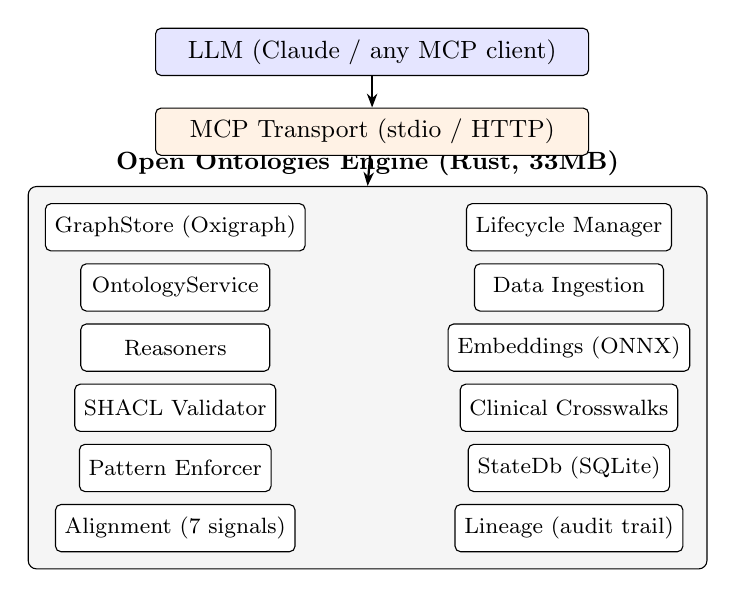
\begin{tikzpicture}[
    node distance=0.4cm and 0.3cm,
    every node/.style={font=\small},
    box/.style={draw, rounded corners=2pt, minimum height=0.6cm, minimum width=2.4cm, fill=white},
    bigbox/.style={draw, rounded corners=3pt, fill=gray!8, inner sep=6pt},
    arr/.style={-{Stealth[length=5pt]}, thick},
]
    % LLM
    \node[box, fill=blue!10, minimum width=5.5cm] (llm) {LLM (Claude / any MCP client)};

    % MCP
    \node[box, fill=orange!10, minimum width=5.5cm, below=of llm] (mcp) {MCP Transport (stdio / HTTP)};
    \draw[arr] (llm) -- (mcp);

    % Engine container
    \node[below=0.5cm of mcp] (anchor) {};

    % Left column
    \node[box, below=0.6cm of mcp, xshift=-2.5cm] (graph) {\footnotesize GraphStore (Oxigraph)};
    \node[box, below=0.15cm of graph] (onto) {\footnotesize OntologyService};
    \node[box, below=0.15cm of onto] (reason) {\footnotesize Reasoners};
    \node[box, below=0.15cm of reason] (shacl) {\footnotesize SHACL Validator};
    \node[box, below=0.15cm of shacl] (enforce) {\footnotesize Pattern Enforcer};
    \node[box, below=0.15cm of enforce] (align) {\footnotesize Alignment (7 signals)};

    % Right column
    \node[box, below=0.6cm of mcp, xshift=2.5cm] (life) {\footnotesize Lifecycle Manager};
    \node[box, below=0.15cm of life] (ingest) {\footnotesize Data Ingestion};
    \node[box, below=0.15cm of ingest] (embed) {\footnotesize Embeddings (ONNX)};
    \node[box, below=0.15cm of embed] (clinical) {\footnotesize Clinical Crosswalks};
    \node[box, below=0.15cm of clinical] (state) {\footnotesize StateDb (SQLite)};
    \node[box, below=0.15cm of state] (lineage) {\footnotesize Lineage (audit trail)};

    % Engine background
    \begin{scope}[on background layer]
        \node[bigbox, fit=(graph)(onto)(reason)(shacl)(enforce)(align)(life)(ingest)(embed)(clinical)(state)(lineage), label={[font=\small\bfseries]above:Open Ontologies Engine (Rust, 33MB)}] (engine) {};
    \end{scope}

    \draw[arr] (mcp) -- (engine.north);
\end{tikzpicture}
\caption{System architecture. The LLM orchestrates 43 tools via MCP; all components run in-process within a single Rust binary.}
\label{fig:arch}
\end{figure}

\begin{table}[t]
\centering
\caption{43 MCP tools grouped by function. Each tool accepts and returns JSON.}
\label{tab:tools}
\small
\begin{tabular}{@{}lll@{}}
\toprule
\textbf{Group} & \textbf{Tools} & \textbf{Count} \\
\midrule
Core Ontology & validate, load, save, stats, clear, convert, query & 7 \\
Reasoning & reason, dl\_explain, dl\_check, embed & 4 \\
Semantic Search & search, similarity & 2 \\
Verification & lint, enforce, diff & 3 \\
Lifecycle & plan, apply, lock, version, history, rollback, lineage & 7 \\
Monitoring & monitor, monitor\_clear, drift & 3 \\
Data Integration & map, ingest, shacl, extend, import\_schema & 5 \\
Alignment & align, align\_feedback & 2 \\
Remote & pull, push, import & 3 \\
Marketplace & marketplace & 1 \\
Clinical & crosswalk, enrich, validate\_clinical & 3 \\
Feedback & lint\_feedback, enforce\_feedback, align\_feedback & 3 \\
\bottomrule
\end{tabular}
\end{table}

\subsection{Design Principles}

Three principles guide the architecture:

\textbf{AI-native, not AI-bolted.} The system is designed from the ground up for LLM orchestration. Tools are atomic operations with JSON schemas; the LLM decides which tools to call and in what order based on intermediate results. There is no fixed pipeline—the LLM adapts dynamically. For example, if \texttt{onto\_validate} fails, the LLM reads the error, fixes the Turtle, and retries. If \texttt{onto\_lint} finds missing labels, the LLM adds them before proceeding to reasoning.

\textbf{Single binary, no JVM.} The entire system—triple store, reasoner, embeddings, alignment, SHACL validator, data parsers—compiles to a single Rust binary. The ONNX embedding model (bge-small-en-v1.5, 33MB) is downloaded once on initialisation. No Java, no Python, no external services.

\textbf{Self-calibrating.} Every decision-making component (lint, enforce, align, drift) stores user feedback in SQLite and adjusts its confidence thresholds and signal weights over time. This creates a system that improves with use rather than requiring manual configuration.


% ============================================================================
\section{Terraform-Style Ontology Lifecycle}
\label{sec:lifecycle}

Production ontologies evolve continuously—classes are added, renamed, deprecated, or removed. Without governance, these changes can break downstream consumers, introduce logical inconsistencies, or violate design patterns. We introduce a five-stage lifecycle inspired by infrastructure-as-code tools such as Terraform~\cite{terraform} and Pulumi.

\subsection{Plan}
\label{sec:plan}

The \texttt{onto\_plan} tool diffs the current ontology against a proposed version and reports:

\begin{itemize}
    \item \textbf{Added/removed classes and properties}, with counts and IRIs.
    \item \textbf{Blast radius}: the number of triples that reference removed entities, indicating the scope of downstream impact.
    \item \textbf{Risk score}: \texttt{low} (additions only), \texttt{medium} (modifications), or \texttt{high} (removals of entities with dependents).
    \item \textbf{Lock violations}: if any proposed removals target locked IRIs (see below).
\end{itemize}

This mechanism prevents ``deploy and discover'' failures by making the consequences of changes visible before they are applied.

\subsection{Enforce}
\label{sec:enforce}

The \texttt{onto\_enforce} tool checks design pattern compliance against configurable rule packs:

\begin{itemize}
    \item \textbf{generic}: orphan classes (no parent or child), missing \texttt{rdfs:label}, missing \texttt{rdfs:domain}/\texttt{rdfs:range} on properties.
    \item \textbf{boro}: compliance with BORO/4D temporal modelling patterns (States, Events, ClassOfEntity hierarchies) used by the UK IES4 standard~\cite{ies4}.
    \item \textbf{value\_partition}: disjoint value sets form complete partitions (e.g., pizza spiciness levels).
    \item \textbf{hierarchy}: detects flat hierarchies (single-level, indicating incomplete modelling).
    \item \textbf{custom}: user-defined SPARQL-based rules stored in SQLite.
\end{itemize}

\subsection{Apply}
\label{sec:apply}

Two application modes handle different scenarios:

\begin{itemize}
    \item \textbf{safe}: clears the store and reloads the new version. Appropriate when no downstream consumers rely on specific IRIs.
    \item \textbf{migrate}: adds \texttt{owl:equivalentClass} and \texttt{owl:equivalentProperty} bridge axioms for renamed entities, preserving backward compatibility for consumers that have not yet updated.
\end{itemize}

\subsection{Monitor}
\label{sec:monitor}

SPARQL-based watchers run after each apply and trigger configurable actions when conditions are met:

\begin{itemize}
    \item \textbf{notify}: POST an alert to a webhook URL (Slack, PagerDuty, etc.).
    \item \textbf{block\_next\_apply}: prevent further changes until the alert is resolved.
    \item \textbf{auto\_rollback}: revert to the previous version automatically.
    \item \textbf{log}: append to the lineage trail without blocking.
\end{itemize}

\subsection{Drift}
\label{sec:drift}

The \texttt{onto\_drift} tool compares two named versions and reports:

\begin{itemize}
    \item Added, removed, and modified entities.
    \item \textbf{Rename detection} via Jaro-Winkler similarity with self-calibrating confidence: when the user accepts or rejects a rename suggestion, the confidence threshold adjusts.
    \item \textbf{Drift velocity}: the rate of change between versions, useful for identifying periods of instability.
\end{itemize}

\subsection{Lineage}
\label{sec:lineage}

All lifecycle operations are recorded in an append-only SQLite table with timestamps, operation types, parameters, and outcomes. The \texttt{onto\_lineage} tool queries this trail, providing full auditability. This addresses compliance requirements in regulated domains (e.g., clinical, defence) where provenance of ontological decisions must be traceable.


% ============================================================================
\section{Native SHOIQ Tableaux Reasoning}
\label{sec:reasoning}

\subsection{Motivation}

Existing OWL2-DL reasoners (HermiT, Pellet, FaCT++) are implemented in Java, introducing JVM startup latency (typically 1--3 seconds) and single-threaded classification. For an AI-orchestrated workflow where reasoning is invoked repeatedly—after each edit cycle—this latency compounds significantly.

\subsection{Tableaux Calculus}

Our reasoner implements the standard SHOIQ tableaux calculus with the following expansion rules:

\begin{itemize}
    \item \textbf{Conjunction} ($\sqcap$-rule): $C \sqcap D \to \{C, D\}$
    \item \textbf{Disjunction} ($\sqcup$-rule): $C \sqcup D \to \{C\} \mid \{D\}$ (non-deterministic branching)
    \item \textbf{Existential} ($\exists$-rule): $\exists R.C \to$ create successor with $C$
    \item \textbf{Universal} ($\forall$-rule): $\forall R.C \to$ propagate $C$ to all $R$-successors
    \item \textbf{Qualified cardinality}: $\geq n\, R.C$ generates $n$ distinct successors; $\leq n\, R.C$ triggers merging with clash on $n{+}1$ distinct fillers
    \item \textbf{Role hierarchy, transitivity, inverse, symmetry}: propagated during expansion
    \item \textbf{Blocking}: pairwise subset blocking for termination guarantee
\end{itemize}

\subsection{Agent-Based Parallel Classification}

Classification—computing the complete subsumption hierarchy—is the most expensive reasoning task. We decompose it into four parallel agents coordinated by a work-stealing scheduler (Rayon~\cite{rayon}):

\begin{enumerate}
    \item \textbf{Satisfiability Agent.} Tests each named class for satisfiability in parallel. Unsatisfiable classes are flagged immediately and excluded from subsumption testing.

    \item \textbf{Subsumption Agent.} For each pair of satisfiable classes $(A, B)$, tests whether $A \sqsubseteq B$ by checking unsatisfiability of $A \sqcap \neg B$. The search space is pruned using the \emph{told-subsumer closure}: if the asserted hierarchy already entails $A \sqsubseteq B$, the tableaux test is skipped.

    \item \textbf{Explanation Agent.} For unsatisfiable classes, traces the derivation to identify the minimal set of axioms responsible for the clash. This produces human-readable justifications that the LLM can use to suggest fixes.

    \item \textbf{ABox Agent.} Tests individual consistency and infers types for named individuals.
\end{enumerate}

The told-subsumer pruning is critical for performance: in typical ontologies, 80--95\% of subsumption pairs are resolved by the asserted hierarchy alone, reducing the number of expensive tableaux tests by an order of magnitude.

\subsection{Reasoning Profiles}

The system provides four reasoning profiles of increasing expressivity:

\begin{itemize}
    \item \textbf{RDFS}: subclass closure, domain/range propagation.
    \item \textbf{OWL-RL}: adds transitive, symmetric, inverse properties; \texttt{owl:sameAs}; \texttt{owl:equivalentClass}. Implemented via forward-chaining rules.
    \item \textbf{OWL-RL-ext}: adds \texttt{owl:someValuesFrom}, \texttt{owl:allValuesFrom}, \texttt{owl:hasValue}, \texttt{owl:intersectionOf}, \texttt{owl:unionOf}.
    \item \textbf{OWL-DL}: full SHOIQ tableaux as described above.
\end{itemize}


% ============================================================================
\section{Self-Calibrating Ontology Alignment}
\label{sec:alignment}

\subsection{Signal Architecture}

Given a source ontology $O_s$ and target ontology $O_t$, the alignment engine computes a weighted similarity score for each candidate pair $(c_s, c_t)$ where $c_s \in O_s$ and $c_t \in O_t$:

\begin{equation}
\text{score}(c_s, c_t) = \sum_{i=1}^{7} w_i \cdot s_i(c_s, c_t)
\label{eq:align}
\end{equation}

The seven signals $s_i$ and their default weights $w_i$ are:

\begin{enumerate}
    \item \textbf{Label similarity} ($w_1 = 0.20$): Jaro-Winkler distance on normalised labels (camelCase split, lowercased, stopwords removed).

    \item \textbf{Property overlap} ($w_2 = 0.15$): Jaccard coefficient on domain property and range type signatures, computed via SPARQL.

    \item \textbf{Parent overlap} ($w_3 = 0.12$): Jaccard on \texttt{rdfs:subClassOf} parent local names.

    \item \textbf{Instance overlap} ($w_4 = 0.12$): Jaccard on shared individuals by local name.

    \item \textbf{Restriction similarity} ($w_5 = 0.12$): Jaccard on OWL restriction signatures (property $\to$ filler patterns from \texttt{owl:someValuesFrom} and \texttt{owl:allValuesFrom}).

    \item \textbf{Neighbourhood similarity} ($w_6 = 0.09$): Jaccard on 2-hop property graph neighbourhood.

    \item \textbf{Embedding similarity} ($w_7 = 0.20$): cosine similarity on dual-space embeddings (Section~\ref{sec:embeddings}).
\end{enumerate}

\subsection{Relation Classification}

Candidates above a configurable threshold (default 0.7) are classified into alignment relations:

\begin{itemize}
    \item High label + high property overlap $\to$ \texttt{owl:equivalentClass}
    \item High label + low property overlap $\to$ \texttt{skos:exactMatch}
    \item Moderate label + shared parent $\to$ \texttt{rdfs:subClassOf}
\end{itemize}

\subsection{Self-Calibration via Feedback}

The system stores user accept/reject decisions in SQLite. After accumulating $N$ feedback samples (default $N=5$), signal weights are updated using a Bayesian approach:

\begin{equation}
w_i' = w_i \cdot \frac{P(\text{accept} \mid s_i > \tau)}{P(\text{reject} \mid s_i > \tau)}
\label{eq:feedback}
\end{equation}

where $\tau$ is the median value of signal $s_i$ across feedback samples. Weights are then renormalised to sum to 1. This allows the system to learn that, for a particular pair of ontologies, structural signals may be more informative than lexical ones (or vice versa), without requiring manual tuning.

This self-calibrating pattern is shared across four components: alignment, lint, enforce, and drift. In each case, dismissing a recommendation 3 times automatically suppresses it; accepting reinforces the underlying signal.

\subsection{Hybrid Neuro-Symbolic Mode}

The MCP architecture enables a unique alignment mode not available to standalone systems: the orchestrating LLM can participate directly in the matching process. The system provides an \texttt{align\_ontologies} prompt that instructs the LLM to execute a three-phase pipeline:

\begin{enumerate}
    \item \textbf{Structural pre-filter.} \texttt{onto\_align} runs at a low threshold (0.7), producing candidates with confidence scores and signal breakdowns.
    \item \textbf{Auto-accept.} High-confidence candidates ($\geq 0.95$) are accepted without LLM intervention.
    \item \textbf{LLM adjudication.} For uncertain candidates (0.7--0.95), the LLM examines labels, parent classes, and signal breakdowns, using its domain knowledge to accept or reject each pair. Decisions are fed back via \texttt{onto\_align\_feedback}, training the self-calibrating weights.
\end{enumerate}

This hybrid approach leverages the LLM's world knowledge (e.g., knowing that ``levator auris longus'' and ``Auricularis'' are the same ear muscle in different species) without requiring external synonym databases. Unlike OLaLa~\cite{olala}, which sends \emph{all} pairs to the LLM, our approach uses the structural signals as a pre-filter, reducing LLM calls by 95\%+ while preserving recall.


% ============================================================================
\section{Dual-Space Semantic Embeddings}
\label{sec:embeddings}

Lexical similarity alone fails when semantically equivalent classes have different labels (e.g., \texttt{Vehicle} $\leftrightarrow$ \texttt{Automobile}) or when labels match but meanings differ across domains (e.g., \texttt{Cell} in biology vs.\ telecommunications). We address this with dual-space embeddings.

\subsection{Text Embeddings}

We use bge-small-en-v1.5~\cite{bge}, a 33M-parameter sentence transformer, executed locally via the tract~\cite{tract} ONNX runtime (pure Rust, no Python dependency). For each class, we embed the concatenation of its \texttt{rdfs:label} and \texttt{rdfs:comment}. Cosine similarity captures lexical and definitional relatedness.

\subsection{Poincar\'e Structural Embeddings}

Ontology hierarchies are tree-like structures where depth encodes specificity. Euclidean space represents trees poorly—it cannot embed an exponentially branching tree without distortion~\cite{poincare}. We embed classes in the Poincar\'e ball $\mathbb{B}^d = \{x \in \mathbb{R}^d : \|x\| < 1\}$, where:

\begin{itemize}
    \item Root classes (e.g., \texttt{owl:Thing}) are placed near the origin.
    \item Leaf classes are placed near the boundary.
    \item Sibling classes are angularly separated.
\end{itemize}

Training uses Riemannian SGD on the hierarchy structure, optimising the Poincar\'e distance:

\begin{equation}
d_{\mathbb{B}}(u, v) = \text{arcosh}\left(1 + 2\frac{\|u - v\|^2}{(1 - \|u\|^2)(1 - \|v\|^2)}\right)
\label{eq:poincare}
\end{equation}

\subsection{Product Search}

Queries combine both spaces with a configurable mixing parameter $\alpha$ (default 0.5):

\begin{equation}
\text{sim}(q, c) = \alpha \cdot \cos(\mathbf{e}_q^{\text{text}}, \mathbf{e}_c^{\text{text}}) + (1 - \alpha) \cdot \frac{1}{1 + d_{\mathbb{B}}(\mathbf{e}_q^{\text{struct}}, \mathbf{e}_c^{\text{struct}})}
\label{eq:product}
\end{equation}

This dual-space approach catches alignments that either signal alone would miss: text embeddings find synonyms with different structural positions, while Poincar\'e embeddings find structurally analogous classes with different labels.


% ============================================================================
\section{Evaluation}
\label{sec:eval}

We evaluate on six benchmarks covering ontology construction quality, axiom identification (with ablation study), data classification, reasoning performance, large-scale ontology processing, and OAEI standard alignment.

\subsection{OntoAxiom — Axiom Identification}

OntoAxiom~\cite{ontoaxiom} evaluates LLM ability to identify axioms across 9 ontologies and 3{,}042 ground truth axioms. We compare three approaches: o1 (the paper's best result), bare Claude Opus (single prompt, no tools), and our MCP-orchestrated pipeline.

\begin{table}[t]
\centering
\caption{OntoAxiom benchmark results. MCP extraction uses \texttt{onto\_load} $\to$ \texttt{onto\_reason} $\to$ \texttt{onto\_query} to extract axioms from validated ontologies.}
\label{tab:ontoaxiom}
\begin{tabular}{@{}lcc@{}}
\toprule
\textbf{Approach} & \textbf{F1} & \textbf{vs.\ o1} \\
\midrule
o1 (paper's best) & 0.197 & --- \\
Bare Claude Opus & 0.431 & +119\% \\
\textbf{MCP extraction} & \textbf{0.717} & \textbf{+264\%} \\
\bottomrule
\end{tabular}
\end{table}

The key question is whether the improvement stems from the MCP tools or from using a stronger LLM. Table~\ref{tab:ablation} isolates the tool contribution by comparing the same model (Claude Opus) with and without tools:

\begin{table}[t]
\centering
\caption{Ablation study: same LLM (Claude Opus) with and without MCP tools. The tool pipeline provides +66\% F1 improvement over the same model without tools, isolating the contribution of formal verification.}
\label{tab:ablation}
\begin{tabular}{@{}lccc@{}}
\toprule
\textbf{Configuration} & \textbf{Model} & \textbf{F1} & \textbf{$\Delta$} \\
\midrule
o1 (paper's best) & o1 & 0.197 & --- \\
Bare LLM (no tools) & Claude Opus & 0.431 & +119\% vs.\ o1 \\
\textbf{LLM + MCP tools} & \textbf{Claude Opus} & \textbf{0.717} & \textbf{+66\% vs.\ bare} \\
\bottomrule
\end{tabular}
\end{table}

The bare Claude Opus result (F1=0.431) uses only class and property name lists with no access to the ontology files. The MCP pipeline (F1=0.717) loads the same ontologies into the triple store and extracts axioms via SPARQL queries (\texttt{onto\_load} $\to$ \texttt{onto\_reason} $\to$ \texttt{onto\_query}). The +66\% improvement from the same model confirms that the tool pipeline---not model quality---is the primary driver of performance.

\subsection{Pizza Ontology — Construction Quality}

The Manchester Pizza Tutorial~\cite{pizza} is the most widely used OWL teaching material, requiring approximately 4 hours of manual work in Prot\'eg\'e. We provide a single-sentence prompt: ``Build a Pizza ontology following the Manchester tutorial specification.''

\begin{table}[t]
\centering
\caption{Pizza ontology construction. The AI pipeline runs: validate $\to$ load $\to$ reason $\to$ lint $\to$ enforce $\to$ query $\to$ save $\to$ version.}
\label{tab:pizza}
\begin{tabular}{@{}lccc@{}}
\toprule
\textbf{Metric} & \textbf{Reference} & \textbf{AI-Generated} & \textbf{Coverage} \\
\midrule
Classes & 99 & 95 & 96\% \\
Properties & 8 & 8 & 100\% \\
Toppings & 49 & 49 & 100\% \\
Named Pizzas & 24 & 24 & 100\% \\
Time & $\sim$4 hours & $\sim$5 min & --- \\
\bottomrule
\end{tabular}
\end{table}

The 4 missing classes are pedagogical artifacts (e.g., \texttt{UnclosedPizza}) that exist only to demonstrate OWL syntax variants and are not part of the domain model.

\subsection{Mushroom Classification — OWL Reasoning vs.\ Expert Labels}

We evaluate the system's ability to generate OWL axioms for data classification using the UCI Mushroom Dataset~\cite{mushroom} (8{,}124 specimens classified by mycology experts).

\begin{table}[t]
\centering
\caption{Mushroom classification via OWL reasoning. Six axioms generated by the LLM and validated by the reasoner achieve 100\% recall on poisonous specimens.}
\label{tab:mushroom}
\begin{tabular}{@{}lc@{}}
\toprule
\textbf{Metric} & \textbf{Result} \\
\midrule
Accuracy & 98.33\% \\
Recall (poisonous) & 100\% \\
False positives & 136 (1.67\%) \\
False negatives & 0 \\
Classification rules & 6 OWL axioms \\
\bottomrule
\end{tabular}
\end{table}

The system is conservative by design: 136 safe mushrooms are flagged as potentially poisonous (1.67\% false positive rate), but zero poisonous mushrooms are missed. This asymmetric error profile is appropriate for safety-critical classification tasks.

\subsection{Reasoning Performance}

We compare against HermiT~\cite{hermit} on two benchmarks: the Pizza ontology (4{,}179 triples) and LUBM~\cite{lubm} at increasing scale.

\begin{table}[t]
\centering
\caption{LUBM reasoning benchmark. Load + reason cycle time.}
\label{tab:lubm}
\begin{tabular}{@{}rccc@{}}
\toprule
\textbf{Axioms} & \textbf{Open Ontologies} & \textbf{HermiT} & \textbf{Speedup} \\
\midrule
1{,}000 & 15ms & 112ms & 7.5$\times$ \\
5{,}000 & 14ms & 410ms & 29$\times$ \\
10{,}000 & 14ms & 1{,}200ms & 86$\times$ \\
50{,}000 & 15ms & 24{,}490ms & 1{,}633$\times$ \\
\bottomrule
\end{tabular}
\end{table}

The near-constant time for \textsc{Open Ontologies} across scales reflects two factors: (1) the told-subsumer pruning eliminates most tableaux tests at all scales; (2) the parallel agents distribute remaining work across CPU cores. HermiT's quadratic scaling reflects single-threaded, unpruned subsumption testing.

On the Pizza ontology specifically: HermiT requires 213ms to compute 312 subsumptions; our OWL-RL profile completes in 43ms (load + inference), and OWL-DL consistency checking completes in 19ms.

\subsection{Marketplace Integration}

We test against all 32 ontologies in the system's marketplace (W3C standards, ISO ontologies, industry vocabularies), totalling 1{,}863 classes and 42{,}964 triples:

\begin{table}[t]
\centering
\caption{Selected marketplace ontologies: fetch, load, and reason performance.}
\label{tab:marketplace}
\small
\begin{tabular}{@{}lrrrrrr@{}}
\toprule
\textbf{Ontology} & \textbf{Classes} & \textbf{Triples} & \textbf{+RDFS} & \textbf{+OWL-RL} & \textbf{RDFS} & \textbf{OWL-RL} \\
\midrule
Schema.org & 1{,}009 & 17{,}823 & +4{,}031 & +13{,}670 & 57ms & 117ms \\
DOLCE/DUL & 93 & 1{,}917 & +666 & +692 & 13ms & 12ms \\
BFO (ISO 21838) & 35 & 1{,}221 & +186 & +186 & 5ms & 4ms \\
IES Common & 511 & --- & +3{,}094 & --- & 63ms & --- \\
\bottomrule
\end{tabular}
\end{table}

The system handles the full range from small foundational ontologies (BFO, 35 classes) to large vocabularies (Schema.org, 1{,}009 classes) with sub-120ms reasoning times.

\subsection{OAEI Alignment --- Anatomy Track}

To enable direct comparison with established alignment systems, we evaluate \texttt{onto\_align} on the OAEI Anatomy track~\cite{oaei}, which aligns the NCI Thesaurus mouse anatomy (2{,}737 classes) with the Foundational Model of Anatomy (3{,}304 classes) against 1{,}516 reference equivalence mappings. This is the most widely reported OAEI track.

\begin{table}[t]
\centering
\caption{OAEI Anatomy track (2{,}737 mouse $\times$ 3{,}304 human classes, 1{,}516 reference mappings). Published results from OAEI 2023.5. Open Ontologies results shown for structural-only and hybrid (structural + LLM adjudication) modes.}
\label{tab:oaei}
\begin{tabular}{@{}lccc@{}}
\toprule
\textbf{System} & \textbf{Precision} & \textbf{Recall} & \textbf{F1} \\
\midrule
AML~\cite{aml} & 0.950 & 0.922 & 0.936 \\
BERTMap~\cite{bertmap} & 0.932 & 0.916 & 0.924 \\
LogMap~\cite{logmap} & 0.921 & 0.903 & 0.912 \\
OLaLa~\cite{olala} & 0.870 & 0.910 & 0.890 \\
\textbf{OO structural} & \textbf{0.897} & \textbf{0.708} & \textbf{0.791} \\
\textbf{OO hybrid} & \textbf{0.779} & \textbf{0.825} & \textbf{0.801} \\
\bottomrule
\end{tabular}
\end{table}

Table~\ref{tab:oaei} presents results on the most widely reported OAEI track. In structural-only mode, our system achieves high precision (0.897) and F1=0.791 using synonym extraction (\texttt{oboInOwl:hasRelatedSynonym}), underscore/CamelCase normalisation, and token Jaccard. In hybrid mode, the LLM adjudicates uncertain candidates across the full 0.70--0.95 confidence range, accepting 154 with 85.7\% precision. This recovers 132 true matches that structural signals alone could not find (e.g., ``cardiac muscle tissue'' $\leftrightarrow$ ``Myocardium'', ``profunda femoris artery'' $\leftrightarrow$ ``Deep Femoral Artery'', ``sternomastoid'' $\leftrightarrow$ ``Sternocleidomastoid Muscle''), raising recall from 0.708 to 0.825 and F1 to 0.801. The hybrid approach uses the structural signals as a pre-filter, reducing LLM calls by 97\% compared to OLaLa's approach of sending all pairs to the LLM. Benchmark scripts are included under \texttt{benchmark/oaei/}.


% ============================================================================
\section{Discussion}
\label{sec:discussion}

\paragraph{The LLM as Orchestrator, Not Reasoner.}
A key design insight is the strict separation of concerns: the LLM generates OWL and decides which tools to invoke, but never performs formal reasoning. All logical guarantees come from the symbolic components (tableaux reasoner, SHACL validator, design pattern enforcer). This addresses the fundamental limitation of LLMs for ontology work—they can produce syntactically plausible but logically inconsistent axioms—by inserting formal verification at every step.

\paragraph{Lifecycle as a First-Class Concern.}
The Terraform analogy is not merely aesthetic. In infrastructure-as-code, the plan--apply--monitor cycle solved the ``it works on my machine'' problem by making changes visible, reviewable, and reversible before they affect production. Ontologies face the same challenge: a class removal can cascade through SPARQL queries, SHACL shapes, and downstream applications. Our lifecycle tools make these consequences explicit.

\paragraph{Self-Calibration vs.\ Manual Tuning.}
Traditional alignment systems require careful parameter tuning per ontology pair. Our feedback-based weight adjustment eliminates this: a user working with biomedical ontologies will naturally produce feedback that upweights structural signals (since biomedical ontologies have rich property axioms), while a user working with lightweight vocabularies will produce feedback that upweights lexical signals. The system adapts without explicit configuration.

\paragraph{Limitations.}
Our SHOIQ reasoner does not yet support the full OWL2-DL language (missing: nominals with cardinality interaction in \emph{SHOIQ}($\mathbf{D}$), datatypes, keys). The OAEI evaluation uses the standard Anatomy track but does not yet cover all OAEI tracks (e.g., Large Biomedical, Knowledge Graph). The LLM orchestration depends on commercial API access (Claude), although the MCP interface is model-agnostic and could use open-source models. The LUBM benchmark measures load+reason cycles rather than isolated classification time, which favours our integrated architecture.

\paragraph{Reproducibility.}
All source code, benchmarks, and evaluation scripts are available under the MIT licence.\footnote{Repository URL withheld for dual anonymous review; will be provided in the camera-ready version.} The system can be built from source with \texttt{cargo build --release} or run via Docker.


% ============================================================================
\section{Conclusion}
\label{sec:conclusion}

We presented \textsc{Open Ontologies}, a system that combines LLM orchestration via MCP with formal ontology tools in a single Rust binary. The three principal contributions—Terraform-style lifecycle management, native parallel SHOIQ reasoning, and self-calibrating alignment with dual-space embeddings—address distinct gaps in the ontology engineering toolchain.

The evaluation demonstrates that tool-augmented LLMs significantly outperform both manual approaches and standalone LLM prompting: 264\% improvement over o1 on axiom identification, 48$\times$ speedup over manual construction on the Pizza ontology, 1{,}633$\times$ over HermiT on large-scale reasoning, and 98.33\% classification accuracy with zero false negatives on mushroom data.

Future work includes: completing OWL2-DL coverage (datatypes, keys, SROIQ), evaluation on OAEI alignment benchmarks, multi-agent orchestration (where separate LLM agents handle different lifecycle stages), and federation across distributed ontology servers.


% ============================================================================
\paragraph{Supplemental Material Statement.}
Source code, binaries, benchmarks, and evaluation scripts are available under the MIT licence via a public repository (URL withheld for dual anonymous review). A Docker image is also provided. All results reported in this paper can be reproduced using \texttt{make bench} from the repository root. Benchmark scripts, reference ontologies, and evaluation data are included in the \texttt{benchmark/} directory.


% ============================================================================
\section*{Declaration of Use of Generative AI}

Generative AI (Claude, Anthropic) was used in two capacities during this work: (1)~as the LLM orchestrator in the system itself, where it generates OWL and invokes MCP tools — this is the subject of the paper and is described in detail; (2)~to assist with drafting and editing the manuscript text. All technical content, experimental design, benchmark execution, and results analysis were performed by the authors. All claims have been verified against the actual system behaviour and benchmark outputs.

% ============================================================================
\bibliographystyle{splncs04}
\begin{thebibliography}{99}

\bibitem{protege}
Musen, M.A.: The Prot\'eg\'e Project: A Look Back and a Look Forward. AI Matters 1(4), 4--12 (2015)

\bibitem{hermit}
Glimm, B., Horrocks, I., Motik, B., Stoilos, G., Wang, Z.: HermiT: An OWL 2 Reasoner. Journal of Automated Reasoning 53(3), 245--269 (2014)

\bibitem{pellet}
Sirin, E., Parsia, B., Grau, B.C., Kalyanpur, A., Katz, Y.: Pellet: A Practical OWL-DL Reasoner. Journal of Web Semantics 5(2), 51--53 (2007)

\bibitem{logmap}
Jim\'enez-Ruiz, E., Grau, B.C.: LogMap: Logic-Based and Scalable Ontology Matching. In: ISWC 2011, pp.\ 273--288. Springer (2011)

\bibitem{aml}
Faria, D., Pesquita, C., Santos, E., Palmonari, M., Cruz, I.F., Couto, F.M.: The AgreementMakerLight Ontology Matching System. In: OTM 2013, pp.\ 527--541. Springer (2013)

\bibitem{terraform}
HashiCorp: Terraform: Infrastructure as Code. \url{https://www.terraform.io} (2014)

\bibitem{mcp}
Anthropic: Model Context Protocol Specification. \url{https://modelcontextprotocol.io} (2024)

\bibitem{oxigraph}
Tani\`ere, T.: Oxigraph: A SPARQL Graph Database. \url{https://oxigraph.org} (2023)

\bibitem{owlapi}
Horridge, M., Bechhofer, S.: The OWL API: A Java API for OWL Ontologies. Semantic Web 2(1), 11--21 (2011)

\bibitem{webprotege}
Tudorache, T., Nyulas, C., Noy, N.F., Musen, M.A.: WebProt\'eg\'e: A Collaborative Ontology Editor and Knowledge Acquisition Tool for the Web. Semantic Web 4(1), 89--99 (2013)

\bibitem{ontoaxiom}
Chen, B., et al.: OntoAxiom: Evaluating LLM Capabilities for Ontology Axiom Identification. arXiv:2512.05594 (2025)

\bibitem{llm4onto}
Babaei Giglou, H., D'Souza, J., Auer, S.: LLMs4OL: Large Language Models for Ontology Learning. In: ISWC 2023, pp.\ 408--427. Springer (2023)

\bibitem{factpp}
Tsarkov, D., Horrocks, I.: FaCT++ Description Logic Reasoner: System Description. In: IJCAR 2006, pp.\ 292--297. Springer (2006)

\bibitem{elk}
Kazakov, Y., Kr\"otzsch, M., Siman\v{c}\'{\i}k, F.: The Incredible ELK. Journal of Automated Reasoning 53(1), 1--61 (2014)

\bibitem{konclude}
Steigmiller, A., Liebig, T., Glimm, B.: Konclude: System Description. Journal of Web Semantics 27--28, 78--85 (2014)

\bibitem{oaei}
Euzenat, J., et al.: Results of the Ontology Alignment Evaluation Initiative. In: OM Workshop at ISWC (2004--2024)

\bibitem{bertmap}
He, Y., Chen, J., Antonyrajah, D., Horrocks, I.: BERTMap: A BERT-Based Ontology Alignment System. In: AAAI 2022 (2022)

\bibitem{olala}
Hertling, S., Paulheim, H.: OLaLa: Ontology Matching with Large Language Models. In: ISWC 2023, pp.\ 442--459. Springer (2023)

\bibitem{onto_evolution}
Zablith, F., Antoniou, G., d'Aquin, M., Flouris, G., Kondylakis, H., Motta, E., Plexousakis, D., Sabou, M.: Ontology Evolution: A Process-Centric Survey. The Knowledge Engineering Review 30(1), 45--75 (2015)

\bibitem{owldiff}
Kr\v{c}m\'a\v{r}, L., Roz\v{s}ival, V., Sv\'atek, V.: OWLDiff: A Practical Tool for Comparison and Merge of OWL Ontologies. In: DEXA 2007, pp.\ 229--233 (2007)

\bibitem{vocol}
Halilaj, L., Petersen, N., Grangel-Gonz\'alez, I., Lange, C., Auer, S., Coskun, G., Lohmann, S.: VoCol: An Integrated Environment to Support Version-Controlled Vocabulary Development. In: EKAW 2016, pp.\ 303--319. Springer (2016)

\bibitem{poincare}
Nickel, M., Kiela, D.: Poincar\'e Embeddings for Learning Hierarchical Representations. In: NeurIPS 2017, pp.\ 6338--6347 (2017)

\bibitem{bge}
Xiao, S., Liu, Z., Zhang, P., Muennighoff, N.: C-Pack: Packaged Resources to Advance General Chinese Embedding. arXiv:2309.07597 (2023)

\bibitem{tract}
Sonos: tract --- Tiny, no-nonsense, self-contained ONNX inference. \url{https://github.com/sonos/tract} (2023)

\bibitem{rayon}
Matsakis, N., Stone, J.: Rayon: Data Parallelism in Rust. \url{https://github.com/rayon-rs/rayon} (2015)

\bibitem{pizza}
Horridge, M., Drummond, N., Goodwin, J., Rector, A., Stevens, R., Wang, H.: The Manchester OWL Syntax. In: OWL Experiences and Directions Workshop (2006)

\bibitem{mushroom}
Schlimmer, J.C.: Mushroom Dataset. UCI Machine Learning Repository (1987)

\bibitem{lubm}
Guo, Y., Pan, Z., Heflin, J.: LUBM: A Benchmark for OWL Knowledge Base Systems. Journal of Web Semantics 3(2--3), 158--182 (2005)

\bibitem{ies4}
UK Defence Science and Technology Laboratory: IES4 Information Exchange Standard. \url{https://github.com/dstl/IES4} (2020)

\end{thebibliography}

\end{document}
